% Options for packages loaded elsewhere
\PassOptionsToPackage{unicode}{hyperref}
\PassOptionsToPackage{hyphens}{url}
%
\documentclass[
]{article}
\usepackage{lmodern}
\usepackage{amsmath}
\usepackage{ifxetex,ifluatex}
\ifnum 0\ifxetex 1\fi\ifluatex 1\fi=0 % if pdftex
  \usepackage[T1]{fontenc}
  \usepackage[utf8]{inputenc}
  \usepackage{textcomp} % provide euro and other symbols
  \usepackage{amssymb}
\else % if luatex or xetex
  \usepackage{unicode-math}
  \defaultfontfeatures{Scale=MatchLowercase}
  \defaultfontfeatures[\rmfamily]{Ligatures=TeX,Scale=1}
\fi
% Use upquote if available, for straight quotes in verbatim environments
\IfFileExists{upquote.sty}{\usepackage{upquote}}{}
\IfFileExists{microtype.sty}{% use microtype if available
  \usepackage[]{microtype}
  \UseMicrotypeSet[protrusion]{basicmath} % disable protrusion for tt fonts
}{}
\makeatletter
\@ifundefined{KOMAClassName}{% if non-KOMA class
  \IfFileExists{parskip.sty}{%
    \usepackage{parskip}
  }{% else
    \setlength{\parindent}{0pt}
    \setlength{\parskip}{6pt plus 2pt minus 1pt}}
}{% if KOMA class
  \KOMAoptions{parskip=half}}
\makeatother
\usepackage{xcolor}
\IfFileExists{xurl.sty}{\usepackage{xurl}}{} % add URL line breaks if available
\IfFileExists{bookmark.sty}{\usepackage{bookmark}}{\usepackage{hyperref}}
\hypersetup{
  pdftitle={How to use nma S3 methods},
  hidelinks,
  pdfcreator={LaTeX via pandoc}}
\urlstyle{same} % disable monospaced font for URLs
\usepackage[margin=1in]{geometry}
\usepackage{color}
\usepackage{fancyvrb}
\newcommand{\VerbBar}{|}
\newcommand{\VERB}{\Verb[commandchars=\\\{\}]}
\DefineVerbatimEnvironment{Highlighting}{Verbatim}{commandchars=\\\{\}}
% Add ',fontsize=\small' for more characters per line
\usepackage{framed}
\definecolor{shadecolor}{RGB}{248,248,248}
\newenvironment{Shaded}{\begin{snugshade}}{\end{snugshade}}
\newcommand{\AlertTok}[1]{\textcolor[rgb]{0.94,0.16,0.16}{#1}}
\newcommand{\AnnotationTok}[1]{\textcolor[rgb]{0.56,0.35,0.01}{\textbf{\textit{#1}}}}
\newcommand{\AttributeTok}[1]{\textcolor[rgb]{0.77,0.63,0.00}{#1}}
\newcommand{\BaseNTok}[1]{\textcolor[rgb]{0.00,0.00,0.81}{#1}}
\newcommand{\BuiltInTok}[1]{#1}
\newcommand{\CharTok}[1]{\textcolor[rgb]{0.31,0.60,0.02}{#1}}
\newcommand{\CommentTok}[1]{\textcolor[rgb]{0.56,0.35,0.01}{\textit{#1}}}
\newcommand{\CommentVarTok}[1]{\textcolor[rgb]{0.56,0.35,0.01}{\textbf{\textit{#1}}}}
\newcommand{\ConstantTok}[1]{\textcolor[rgb]{0.00,0.00,0.00}{#1}}
\newcommand{\ControlFlowTok}[1]{\textcolor[rgb]{0.13,0.29,0.53}{\textbf{#1}}}
\newcommand{\DataTypeTok}[1]{\textcolor[rgb]{0.13,0.29,0.53}{#1}}
\newcommand{\DecValTok}[1]{\textcolor[rgb]{0.00,0.00,0.81}{#1}}
\newcommand{\DocumentationTok}[1]{\textcolor[rgb]{0.56,0.35,0.01}{\textbf{\textit{#1}}}}
\newcommand{\ErrorTok}[1]{\textcolor[rgb]{0.64,0.00,0.00}{\textbf{#1}}}
\newcommand{\ExtensionTok}[1]{#1}
\newcommand{\FloatTok}[1]{\textcolor[rgb]{0.00,0.00,0.81}{#1}}
\newcommand{\FunctionTok}[1]{\textcolor[rgb]{0.00,0.00,0.00}{#1}}
\newcommand{\ImportTok}[1]{#1}
\newcommand{\InformationTok}[1]{\textcolor[rgb]{0.56,0.35,0.01}{\textbf{\textit{#1}}}}
\newcommand{\KeywordTok}[1]{\textcolor[rgb]{0.13,0.29,0.53}{\textbf{#1}}}
\newcommand{\NormalTok}[1]{#1}
\newcommand{\OperatorTok}[1]{\textcolor[rgb]{0.81,0.36,0.00}{\textbf{#1}}}
\newcommand{\OtherTok}[1]{\textcolor[rgb]{0.56,0.35,0.01}{#1}}
\newcommand{\PreprocessorTok}[1]{\textcolor[rgb]{0.56,0.35,0.01}{\textit{#1}}}
\newcommand{\RegionMarkerTok}[1]{#1}
\newcommand{\SpecialCharTok}[1]{\textcolor[rgb]{0.00,0.00,0.00}{#1}}
\newcommand{\SpecialStringTok}[1]{\textcolor[rgb]{0.31,0.60,0.02}{#1}}
\newcommand{\StringTok}[1]{\textcolor[rgb]{0.31,0.60,0.02}{#1}}
\newcommand{\VariableTok}[1]{\textcolor[rgb]{0.00,0.00,0.00}{#1}}
\newcommand{\VerbatimStringTok}[1]{\textcolor[rgb]{0.31,0.60,0.02}{#1}}
\newcommand{\WarningTok}[1]{\textcolor[rgb]{0.56,0.35,0.01}{\textbf{\textit{#1}}}}
\usepackage{graphicx}
\makeatletter
\def\maxwidth{\ifdim\Gin@nat@width>\linewidth\linewidth\else\Gin@nat@width\fi}
\def\maxheight{\ifdim\Gin@nat@height>\textheight\textheight\else\Gin@nat@height\fi}
\makeatother
% Scale images if necessary, so that they will not overflow the page
% margins by default, and it is still possible to overwrite the defaults
% using explicit options in \includegraphics[width, height, ...]{}
\setkeys{Gin}{width=\maxwidth,height=\maxheight,keepaspectratio}
% Set default figure placement to htbp
\makeatletter
\def\fps@figure{htbp}
\makeatother
\setlength{\emergencystretch}{3em} % prevent overfull lines
\providecommand{\tightlist}{%
  \setlength{\itemsep}{0pt}\setlength{\parskip}{0pt}}
\setcounter{secnumdepth}{-\maxdimen} % remove section numbering
\ifluatex
  \usepackage{selnolig}  % disable illegal ligatures
\fi

\title{How to use \texttt{nma} S3 methods}
\author{}
\date{\vspace{-2.5em}}

\begin{document}
\maketitle

\hypertarget{introduction}{%
\subsection{Introduction}\label{introduction}}

This document describes how to use the main functions of \texttt{NMA} to
run a network meta-analysis.

\hypertarget{example}{%
\subsection{Example}\label{example}}

\begin{Shaded}
\begin{Highlighting}[]
\FunctionTok{library}\NormalTok{(NMA)}
\FunctionTok{library}\NormalTok{(dplyr)}
\FunctionTok{library}\NormalTok{(purrr)}
\end{Highlighting}
\end{Shaded}

\hypertarget{settings}{%
\subsubsection{Settings}\label{settings}}

Define the BUGS parameters for MCMC.

\begin{Shaded}
\begin{Highlighting}[]
\NormalTok{bugs\_params }\OtherTok{\textless{}{-}}
  \FunctionTok{list}\NormalTok{(}
    \AttributeTok{PROG =} \StringTok{"openBugs"}\NormalTok{,}
    \AttributeTok{N.BURNIN =} \DecValTok{10}\NormalTok{,}\CommentTok{\#00,}
    \AttributeTok{N.SIMS =} \DecValTok{150}\NormalTok{,}\CommentTok{\#0,}
    \AttributeTok{N.CHAINS =} \DecValTok{2}\NormalTok{,}
    \AttributeTok{N.THIN =} \DecValTok{1}\NormalTok{,}
    \AttributeTok{PAUSE =} \ConstantTok{TRUE}\NormalTok{)}
\end{Highlighting}
\end{Shaded}

Define the scenario we will use for the analysis. We will load in a
dataframe of values.

\begin{Shaded}
\begin{Highlighting}[]
\NormalTok{analyses\_params }\OtherTok{\textless{}{-}}
  \FunctionTok{read.csv}\NormalTok{(}
\NormalTok{    here}\SpecialCharTok{::}\FunctionTok{here}\NormalTok{(}\StringTok{"raw\_data"}\NormalTok{, }\StringTok{"AnalysisList.csv"}\NormalTok{),}
    \AttributeTok{as.is =} \ConstantTok{TRUE}\NormalTok{,}
    \AttributeTok{na.strings =} \FunctionTok{c}\NormalTok{(}\StringTok{"NR"}\NormalTok{, }\StringTok{"NA"}\NormalTok{)) }\SpecialCharTok{\%\textgreater{}\%} 
  \FunctionTok{filter}\NormalTok{(Endpoint\_type }\SpecialCharTok{==} \StringTok{"Surv"}\NormalTok{) }\SpecialCharTok{\%\textgreater{}\%} 
\NormalTok{  dplyr}\SpecialCharTok{::}\FunctionTok{rename}\NormalTok{(}\AttributeTok{name =}\NormalTok{ Analysis\_name,}
                \AttributeTok{type =}\NormalTok{ Analysis\_Type)}
\end{Highlighting}
\end{Shaded}

For demonstration purposes we will select the first scenario to run.

\begin{Shaded}
\begin{Highlighting}[]
\NormalTok{analysis }\OtherTok{\textless{}{-}}\NormalTok{ analyses\_params[}\DecValTok{1}\NormalTok{, ]}

\CommentTok{\# fixed effects RANDOM=FALSE, random effects RANDOM=TRUE}
\NormalTok{RANDOM }\OtherTok{\textless{}{-}}\NormalTok{ analysis}\SpecialCharTok{$}\NormalTok{Model\_effects }\SpecialCharTok{==} \StringTok{"RE"}

\NormalTok{REFTX }\OtherTok{\textless{}{-}}\NormalTok{ analysis}\SpecialCharTok{$}\NormalTok{REFTX}

\CommentTok{\# indicator for availability of binary endpoint data}
\NormalTok{is\_bin }\OtherTok{\textless{}{-}}\NormalTok{ analysis}\SpecialCharTok{$}\NormalTok{BinData }\SpecialCharTok{==} \StringTok{"YES"}

\CommentTok{\# indicator for availability of median endpoint data}
\NormalTok{is\_med }\OtherTok{\textless{}{-}}\NormalTok{ analysis}\SpecialCharTok{$}\NormalTok{MedData }\SpecialCharTok{==} \StringTok{"YES"}
\end{Highlighting}
\end{Shaded}

\hypertarget{read-in-datasets}{%
\subsubsection{Read in datasets}\label{read-in-datasets}}

The trials data consist of upto 3 separate dataframes. A main table,
\texttt{subData}, and optional tables for median event time and binary
data, \texttt{subDataMed} and \texttt{subDataBin} respectively.

\begin{Shaded}
\begin{Highlighting}[]
\NormalTok{file\_name }\OtherTok{\textless{}{-}} \FunctionTok{paste0}\NormalTok{(here}\SpecialCharTok{::}\FunctionTok{here}\NormalTok{(}\StringTok{"raw\_data"}\NormalTok{), }\StringTok{"/survdata\_"}\NormalTok{, analysis}\SpecialCharTok{$}\NormalTok{Endpoint, }\StringTok{"\_"}\NormalTok{)}

\NormalTok{subData }\OtherTok{\textless{}{-}}
  \FunctionTok{read.csv}\NormalTok{(}\FunctionTok{paste0}\NormalTok{(file\_name, analysis}\SpecialCharTok{$}\NormalTok{type, }\StringTok{".csv"}\NormalTok{),}
           \AttributeTok{header =} \ConstantTok{TRUE}\NormalTok{,}
           \AttributeTok{as.is =} \ConstantTok{TRUE}\NormalTok{)}

\NormalTok{subDataBin }\OtherTok{\textless{}{-}}
  \ControlFlowTok{if}\NormalTok{ (is\_bin) \{}
    \FunctionTok{read.csv}\NormalTok{(}\FunctionTok{paste0}\NormalTok{(file\_name, }\StringTok{"bin.csv"}\NormalTok{),}
             \AttributeTok{header =} \ConstantTok{TRUE}\NormalTok{,}
             \AttributeTok{as.is =} \ConstantTok{TRUE}\NormalTok{)}
\NormalTok{  \} }\ControlFlowTok{else}\NormalTok{ \{}\ConstantTok{NA}\NormalTok{\}}

\NormalTok{subDataMed }\OtherTok{\textless{}{-}}
  \ControlFlowTok{if}\NormalTok{ (is\_med) \{}
    \FunctionTok{read.csv}\NormalTok{(}\FunctionTok{paste0}\NormalTok{(file\_name, }\StringTok{"med.csv"}\NormalTok{),}
             \AttributeTok{header =} \ConstantTok{TRUE}\NormalTok{,}
             \AttributeTok{as.is =} \ConstantTok{TRUE}\NormalTok{) }\SpecialCharTok{\%\textgreater{}\%} 
      \FunctionTok{mutate}\NormalTok{(}\AttributeTok{medR =} \FunctionTok{floor}\NormalTok{(medR))}
\NormalTok{  \} }\ControlFlowTok{else}\NormalTok{ \{}\ConstantTok{NA}\NormalTok{\}}
\end{Highlighting}
\end{Shaded}

\hypertarget{build-model}{%
\subsubsection{Build model}\label{build-model}}

Now we can create the NMA object to use in the modelling.

\begin{Shaded}
\begin{Highlighting}[]
\NormalTok{nma\_model }\OtherTok{\textless{}{-}}
  \FunctionTok{new\_NMA}\NormalTok{(}\AttributeTok{subData =}\NormalTok{ subData,}
          \AttributeTok{subDataMed =}\NormalTok{ subDataMed,}
          \AttributeTok{subDataBin =}\NormalTok{ subDataBin,}
          \AttributeTok{bugs\_params =}\NormalTok{ bugs\_params,}
          \AttributeTok{is\_random =}\NormalTok{ RANDOM,}
          \AttributeTok{refTx =}\NormalTok{ REFTX ,}
          \AttributeTok{effectParam =} \StringTok{"beta"}\NormalTok{,}
          \AttributeTok{modelParams =} \StringTok{"totresdev"}\NormalTok{,}
          \AttributeTok{label =}\NormalTok{ analysis}\SpecialCharTok{$}\NormalTok{name,}
          \AttributeTok{endpoint =}\NormalTok{ analysis}\SpecialCharTok{$}\NormalTok{Endpoint)}

\NormalTok{nma\_model}
\CommentTok{\#\textgreater{} $dat}
\CommentTok{\#\textgreater{} $dat$inits}
\CommentTok{\#\textgreater{} function() \{}
\CommentTok{\#\textgreater{}       list(}
\CommentTok{\#\textgreater{}         beta = c(NA, rnorm(nTx {-} 1, 0, 2)),}
\CommentTok{\#\textgreater{}         sd = 0.1,}
\CommentTok{\#\textgreater{}         alpha = rnorm(nStudies)) \%\textgreater{}\% }
\CommentTok{\#\textgreater{}         .[param\_names]}
\CommentTok{\#\textgreater{}     \}}
\CommentTok{\#\textgreater{} \textless{}bytecode: 0x00000174580ede80\textgreater{}}
\CommentTok{\#\textgreater{} \textless{}environment: 0x000001745825eed8\textgreater{}}
\CommentTok{\#\textgreater{} }
\CommentTok{\#\textgreater{} $dat$subData}
\CommentTok{\#\textgreater{}     X                                 study                  base            tx       Lmean       Lse multi\_arm Ltx Lbase Lstudy}
\CommentTok{\#\textgreater{} 1   6                ARCHER 1050 (Wu, 2017)               ERL/GEF           DAC {-}0.47803580 0.1134403         0   7     1      6}
\CommentTok{\#\textgreater{} 2   9                   CONVINCE (Shi 2017)               CIS+PEM           ICO {-}0.43078292 0.1546265         0  19     5      9}
\CommentTok{\#\textgreater{} 3  26      CTRI/2015/08/006113 (Patil 2017)             CARBO+PEM       ERL/GEF {-}0.41551544 0.1291164         0   1     4     24}
\CommentTok{\#\textgreater{} 4  15   CTRI/2016/08/007149 (Noronha 2019b)               ERL/GEF GEF+CARBO+PEM {-}0.67330000 0.1342100         0  12     1     13}
\CommentTok{\#\textgreater{} 5  22                      ENSURE (Wu 2015)               GEM+CIS       ERL/GEF {-}1.07880966 0.2144855         0   1    18     20}
\CommentTok{\#\textgreater{} 6   5                   FLAURA (Soria 2018)               ERL/GEF           OSI {-}0.77652879 0.1102381         0  22     1      5}
\CommentTok{\#\textgreater{} 7   4                   GOAL (Campelo 2018)               ERL/GEF       GEF+OLA {-}0.28768207 0.1864509         0  16     1      4}
\CommentTok{\#\textgreater{} 8   3                    INCREASE (Li 2018)                   ICO ICO high{-}dose {-}0.30110509 0.1758496         0  20    19      3}
\CommentTok{\#\textgreater{} 9  17 JO25567 (JapicCTI{-}111390) (Seto 2014)               ERL/GEF       ERL+BEV {-}0.61618614 0.2004921         0   9     1     15}
\CommentTok{\#\textgreater{} 10  2             LUX{-}Lung 3 (Sequist 2013)               CIS+PEM           AFA {-}0.71334989 0.1437422         0   2     5      2}
\CommentTok{\#\textgreater{} 11 24               LUX{-}Lung 6 (Wu 2014a)\textbackslash{}n               GEM+CIS           AFA {-}1.34707365 0.1630306         0   2    18     22}
\CommentTok{\#\textgreater{} 12 25                LUX{-}Lung 7 (Park 2016)               ERL/GEF           AFA {-}0.24846136 0.1235321         0   2     1     23}
\CommentTok{\#\textgreater{} 13 20              NCT01017874 (Yang, 2014)               ERL/GEF CIS+PEM+GEF\_m {-}0.18632958 0.3443691         0   6     1     18}
\CommentTok{\#\textgreater{} 14  7              NCT01221077 (Leighl 2017               ERL/GEF       LIN+ERL  0.31188676 0.2970771         0  21     1      7}
\CommentTok{\#\textgreater{} 15 18              NCT01469000 (Yang, 2020)               ERL/GEF       GEF+PEM {-}0.40047757 0.1499456         0  17     1     16}
\CommentTok{\#\textgreater{} 16 16        NCT01532089 (Stinchcombe 2019)               ERL/GEF       ERL+BEV {-}0.21072103 0.2457077         0   9     1     14}
\CommentTok{\#\textgreater{} 17 21                 NCT01769066 (Yu 2014)               CIS+PEM CIS+PEM+GEF\_m {-}1.60943791 0.6908291         0   6     5     19}
\CommentTok{\#\textgreater{} 18 28                 NCT01864681 (Li 2019)               ERL/GEF       GEF+MET  0.03922071 0.1681749         0  15     1     26}
\CommentTok{\#\textgreater{} 19  8        NCT01897480 (Scagliotti, 2020)               ERL/GEF       EMI+ERL {-}0.11653382 0.1658275         0   8     1      8}
\CommentTok{\#\textgreater{} 20 12               NCT02148380 (Han, 2017)               ERL/GEF     CARBO+PEM  1.04982212 0.4706135         1   4     1     10}
\CommentTok{\#\textgreater{} 21 10               NCT02148380 (Han, 2017)               ERL/GEF       ERL/GEF  0.00000000 0.2152550         1   1     1     10}
\CommentTok{\#\textgreater{} 22 11               NCT02148380 (Han, 2017)               ERL/GEF GEF+CARBO+PEM {-}0.73396918 0.4539455         1  12     1     10}
\CommentTok{\#\textgreater{} 23 13      NEJ005/TCOG0902 (Sugawara, 2015) GEF+CARBO+PEM (Alter) GEF+CARBO+PEM {-}0.34249031 0.2678118         0  12    13     11}
\CommentTok{\#\textgreater{} 24 27  NEJ009 (UMIN000006340) (Hosomi 2019)               ERL/GEF GEF+CARBO+PEM {-}0.71334989 0.1182584         0  12     1     25}
\CommentTok{\#\textgreater{} 25 19                   NEJ026 (Saito 2019)               ERL/GEF       ERL+BEV {-}0.50252682 0.1896482         0   9     1     17}
\CommentTok{\#\textgreater{} 26  1                RELAY (Nakagawa, 2019)               ERL/GEF       RAM+ERL {-}0.52593926 0.1275307         0  23     1      1}
\CommentTok{\#\textgreater{} 27 14            SWOG S1403 (Goldberg 2018)                   AFA       AFA+CET  0.15700375 0.1967513         0   3     2     12}
\CommentTok{\#\textgreater{} 28 23                 TORCH (Gridelli 2012)               GEM+CIS       ERL/GEF {-}0.51082562 0.3536465         0   1    18     21}
\CommentTok{\#\textgreater{} }
\CommentTok{\#\textgreater{} $dat$subDataBin}
\CommentTok{\#\textgreater{}                     study    base      tx BinR BinN Btx Bbase Bstudy}
\CommentTok{\#\textgreater{} 1 NCT01039948 (Mok, 2016) ERL/GEF ERL/GEF   34   38   1     1     33}
\CommentTok{\#\textgreater{} 2 NCT01039948 (Mok, 2016) ERL/GEF GEF+FIC   27   33  14     1     33}
\CommentTok{\#\textgreater{} }
\CommentTok{\#\textgreater{} $dat$subDataMed}
\CommentTok{\#\textgreater{}                                     study          base            tx median medN medR mediantx medianbase medianstudy}
\CommentTok{\#\textgreater{} 1                                 An 2016       ERL/GEF       ERL/GEF   14.0   45   22        1          1          27}
\CommentTok{\#\textgreater{} 2                                 An 2016       ERL/GEF       GEF+PEM   18.0   45   22       17          1          27}
\CommentTok{\#\textgreater{} 3  CALGB 30406 (NCT00126581) (Janne 2012)       ERL/GEF       ERL/GEF   14.1   33   16        1          1          30}
\CommentTok{\#\textgreater{} 4  CALGB 30406 (NCT00126581) (Janne 2012)       ERL/GEF ERL+PAC+CARBO   17.2   33   16       10          1          30}
\CommentTok{\#\textgreater{} 5      GENOA / NCT02319577 (Genova, 2019)       ERL/GEF       ERL/GEF    9.5   21   10        1          1          32}
\CommentTok{\#\textgreater{} 6      GENOA / NCT02319577 (Genova, 2019)       ERL/GEF       VIN+GEF    6.2   23   11       24          1          32}
\CommentTok{\#\textgreater{} 7        IFCT{-}1503 ACE{-}Lung (Cortot 2019)           AFA           AFA   11.1   59   29        2          2          29}
\CommentTok{\#\textgreater{} 8        IFCT{-}1503 ACE{-}Lung (Cortot 2019)           AFA       AFA+CET   12.8   59   29        3          2          29}
\CommentTok{\#\textgreater{} 9                  NCT01502202 (Lee 2016) CIS+PEM+GEF\_m       CIS+PEM    7.8   37   18        5          6          31}
\CommentTok{\#\textgreater{} 10                 NCT01502202 (Lee 2016) CIS+PEM+GEF\_m CIS+PEM+GEF\_m   13.3   39   19        6          6          31}
\CommentTok{\#\textgreater{} 11         UMIN000013586 (Kitagawa, 2019)       ERL/GEF       ERL/GEF   15.1   10    5        1          1          28}
\CommentTok{\#\textgreater{} 12         UMIN000013586 (Kitagawa, 2019)       ERL/GEF       GEF+BEV    5.4    6    3       11          1          28}
\CommentTok{\#\textgreater{} }
\CommentTok{\#\textgreater{} $dat$bugsData}
\CommentTok{\#\textgreater{} $dat$bugsData$Lstudy}
\CommentTok{\#\textgreater{}  [1]  6  9 24 13 20  5  4  3 15  2 22 23 18  7 16 14 19 26  8 10 10 10 11 25 17  1 12 21}
\CommentTok{\#\textgreater{} }
\CommentTok{\#\textgreater{} $dat$bugsData$Ltx}
\CommentTok{\#\textgreater{}  [1]  7 19  1 12  1 22 16 20  9  2  2  2  6 21 17  9  6 15  8  4  1 12 12 12  9 23  3  1}
\CommentTok{\#\textgreater{} }
\CommentTok{\#\textgreater{} $dat$bugsData$Lbase}
\CommentTok{\#\textgreater{}  [1]  1  5  4  1 18  1  1 19  1  5 18  1  1  1  1  1  5  1  1  1  1  1 13  1  1  1  2 18}
\CommentTok{\#\textgreater{} }
\CommentTok{\#\textgreater{} $dat$bugsData$Lmean}
\CommentTok{\#\textgreater{}  [1] {-}0.47803580 {-}0.43078292 {-}0.41551544 {-}0.67330000 {-}1.07880966 {-}0.77652879 {-}0.28768207 {-}0.30110509 {-}0.61618614 {-}0.71334989 {-}1.34707365 {-}0.24846136 {-}0.18632958  0.31188676 {-}0.40047757 {-}0.21072103}
\CommentTok{\#\textgreater{} [17] {-}1.60943791  0.03922071 {-}0.11653382  1.04982212  0.00000000 {-}0.73396918 {-}0.34249031 {-}0.71334989 {-}0.50252682 {-}0.52593926  0.15700375 {-}0.51082562}
\CommentTok{\#\textgreater{} }
\CommentTok{\#\textgreater{} $dat$bugsData$Lse}
\CommentTok{\#\textgreater{}  [1] 0.1134403 0.1546265 0.1291164 0.1342100 0.2144855 0.1102381 0.1864509 0.1758496 0.2004921 0.1437422 0.1630306 0.1235321 0.3443691 0.2970771 0.1499456 0.2457077 0.6908291 0.1681749 0.1658275 0.4706135}
\CommentTok{\#\textgreater{} [21] 0.2152550 0.4539455 0.2678118 0.1182584 0.1896482 0.1275307 0.1967513 0.3536465}
\CommentTok{\#\textgreater{} }
\CommentTok{\#\textgreater{} $dat$bugsData$multi}
\CommentTok{\#\textgreater{}  [1] 0 0 0 0 0 0 0 0 0 0 0 0 0 0 0 0 0 0 0 1 1 1 0 0 0 0 0 0}
\CommentTok{\#\textgreater{} }
\CommentTok{\#\textgreater{} $dat$bugsData$LnObs}
\CommentTok{\#\textgreater{} [1] 28}
\CommentTok{\#\textgreater{} }
\CommentTok{\#\textgreater{} $dat$bugsData$nTx}
\CommentTok{\#\textgreater{} [1] 24}
\CommentTok{\#\textgreater{} }
\CommentTok{\#\textgreater{} $dat$bugsData$nStudies}
\CommentTok{\#\textgreater{} [1] 33}
\CommentTok{\#\textgreater{} }
\CommentTok{\#\textgreater{} $dat$bugsData$medianStudy}
\CommentTok{\#\textgreater{}  [1] 27 27 30 30 32 32 29 29 31 31 28 28}
\CommentTok{\#\textgreater{} }
\CommentTok{\#\textgreater{} $dat$bugsData$medianTx}
\CommentTok{\#\textgreater{}  [1]  1 17  1 10  1 24  2  3  5  6  1 11}
\CommentTok{\#\textgreater{} }
\CommentTok{\#\textgreater{} $dat$bugsData$medianBase}
\CommentTok{\#\textgreater{}  [1] 1 1 1 1 1 1 2 2 6 6 1 1}
\CommentTok{\#\textgreater{} }
\CommentTok{\#\textgreater{} $dat$bugsData$Bstudy}
\CommentTok{\#\textgreater{} [1] 33 33}
\CommentTok{\#\textgreater{} }
\CommentTok{\#\textgreater{} $dat$bugsData$Btx}
\CommentTok{\#\textgreater{} [1]  1 14}
\CommentTok{\#\textgreater{} }
\CommentTok{\#\textgreater{} $dat$bugsData$Bbase}
\CommentTok{\#\textgreater{} [1] 1 1}
\CommentTok{\#\textgreater{} }
\CommentTok{\#\textgreater{} $dat$bugsData$medianN}
\CommentTok{\#\textgreater{}  [1] 45 45 33 33 21 23 59 59 37 39 10  6}
\CommentTok{\#\textgreater{} }
\CommentTok{\#\textgreater{} $dat$bugsData$medianR}
\CommentTok{\#\textgreater{}  [1] 22 22 16 16 10 11 29 29 18 19  5  3}
\CommentTok{\#\textgreater{} }
\CommentTok{\#\textgreater{} $dat$bugsData$median}
\CommentTok{\#\textgreater{}  [1] 14.0 18.0 14.1 17.2  9.5  6.2 11.1 12.8  7.8 13.3 15.1  5.4}
\CommentTok{\#\textgreater{} }
\CommentTok{\#\textgreater{} $dat$bugsData$medianNObs}
\CommentTok{\#\textgreater{} [1] 12}
\CommentTok{\#\textgreater{} }
\CommentTok{\#\textgreater{} $dat$bugsData$Bn}
\CommentTok{\#\textgreater{} [1] 38 33}
\CommentTok{\#\textgreater{} }
\CommentTok{\#\textgreater{} $dat$bugsData$Br}
\CommentTok{\#\textgreater{} [1] 34 27}
\CommentTok{\#\textgreater{} }
\CommentTok{\#\textgreater{} $dat$bugsData$BnObs}
\CommentTok{\#\textgreater{} [1] 2}
\CommentTok{\#\textgreater{} }
\CommentTok{\#\textgreater{} }
\CommentTok{\#\textgreater{} $dat$txList}
\CommentTok{\#\textgreater{}  [1] "ERL/GEF"               "AFA"                   "AFA+CET"               "CARBO+PEM"             "CIS+PEM"               "CIS+PEM+GEF\_m"         "DAC"                   "EMI+ERL"              }
\CommentTok{\#\textgreater{}  [9] "ERL+BEV"               "ERL+PAC+CARBO"         "GEF+BEV"               "GEF+CARBO+PEM"         "GEF+CARBO+PEM (Alter)" "GEF+FIC"               "GEF+MET"               "GEF+OLA"              }
\CommentTok{\#\textgreater{} [17] "GEF+PEM"               "GEM+CIS"               "ICO"                   "ICO high{-}dose"         "LIN+ERL"               "OSI"                   "RAM+ERL"               "VIN+GEF"              }
\CommentTok{\#\textgreater{} }
\CommentTok{\#\textgreater{} }
\CommentTok{\#\textgreater{} $is\_med}
\CommentTok{\#\textgreater{} [1] TRUE}
\CommentTok{\#\textgreater{} }
\CommentTok{\#\textgreater{} $is\_bin}
\CommentTok{\#\textgreater{} [1] TRUE}
\CommentTok{\#\textgreater{} }
\CommentTok{\#\textgreater{} $bugs\_params}
\CommentTok{\#\textgreater{} $bugs\_params$PROG}
\CommentTok{\#\textgreater{} [1] "openBugs"}
\CommentTok{\#\textgreater{} }
\CommentTok{\#\textgreater{} $bugs\_params$N.BURNIN}
\CommentTok{\#\textgreater{} [1] 10}
\CommentTok{\#\textgreater{} }
\CommentTok{\#\textgreater{} $bugs\_params$N.SIMS}
\CommentTok{\#\textgreater{} [1] 150}
\CommentTok{\#\textgreater{} }
\CommentTok{\#\textgreater{} $bugs\_params$N.CHAINS}
\CommentTok{\#\textgreater{} [1] 2}
\CommentTok{\#\textgreater{} }
\CommentTok{\#\textgreater{} $bugs\_params$N.THIN}
\CommentTok{\#\textgreater{} [1] 1}
\CommentTok{\#\textgreater{} }
\CommentTok{\#\textgreater{} $bugs\_params$PAUSE}
\CommentTok{\#\textgreater{} [1] TRUE}
\CommentTok{\#\textgreater{} }
\CommentTok{\#\textgreater{} $bugs\_params$run\_bugs}
\CommentTok{\#\textgreater{} [1] TRUE}
\CommentTok{\#\textgreater{} }
\CommentTok{\#\textgreater{} }
\CommentTok{\#\textgreater{} $bugs\_fn}
\CommentTok{\#\textgreater{} function(...)}
\CommentTok{\#\textgreater{}         bugs(program = "openbugs", ...)}
\CommentTok{\#\textgreater{} \textless{}bytecode: 0x000001745392bbc8\textgreater{}}
\CommentTok{\#\textgreater{} \textless{}environment: 0x000001745e367750\textgreater{}}
\CommentTok{\#\textgreater{} }
\CommentTok{\#\textgreater{} $is\_random}
\CommentTok{\#\textgreater{} [1] FALSE}
\CommentTok{\#\textgreater{} }
\CommentTok{\#\textgreater{} $refTx}
\CommentTok{\#\textgreater{} [1] "ERL/GEF"}
\CommentTok{\#\textgreater{} }
\CommentTok{\#\textgreater{} $effectParam}
\CommentTok{\#\textgreater{} [1] "beta"}
\CommentTok{\#\textgreater{} }
\CommentTok{\#\textgreater{} $modelParams}
\CommentTok{\#\textgreater{} [1] "totresdev"}
\CommentTok{\#\textgreater{} }
\CommentTok{\#\textgreater{} $label}
\CommentTok{\#\textgreater{} [1] "BC\_PFS\_mFE"}
\CommentTok{\#\textgreater{} }
\CommentTok{\#\textgreater{} $endpoint}
\CommentTok{\#\textgreater{} [1] "PFS"}
\CommentTok{\#\textgreater{} }
\CommentTok{\#\textgreater{} attr(,"class")}
\CommentTok{\#\textgreater{} [1] "nma"}
\CommentTok{\#\textgreater{} attr(,"CALL")}
\CommentTok{\#\textgreater{} attr(,"CALL")$subData}
\CommentTok{\#\textgreater{} subData}
\CommentTok{\#\textgreater{} }
\CommentTok{\#\textgreater{} attr(,"CALL")$subDataMed}
\CommentTok{\#\textgreater{} subDataMed}
\CommentTok{\#\textgreater{} }
\CommentTok{\#\textgreater{} attr(,"CALL")$subDataBin}
\CommentTok{\#\textgreater{} subDataBin}
\CommentTok{\#\textgreater{} }
\CommentTok{\#\textgreater{} attr(,"CALL")$bugs\_params}
\CommentTok{\#\textgreater{} bugs\_params}
\CommentTok{\#\textgreater{} }
\CommentTok{\#\textgreater{} attr(,"CALL")$is\_random}
\CommentTok{\#\textgreater{} RANDOM}
\CommentTok{\#\textgreater{} }
\CommentTok{\#\textgreater{} attr(,"CALL")$refTx}
\CommentTok{\#\textgreater{} REFTX}
\CommentTok{\#\textgreater{} }
\CommentTok{\#\textgreater{} attr(,"CALL")$effectParam}
\CommentTok{\#\textgreater{} [1] "beta"}
\CommentTok{\#\textgreater{} }
\CommentTok{\#\textgreater{} attr(,"CALL")$modelParams}
\CommentTok{\#\textgreater{} [1] "totresdev"}
\CommentTok{\#\textgreater{} }
\CommentTok{\#\textgreater{} attr(,"CALL")$label}
\CommentTok{\#\textgreater{} analysis$name}
\CommentTok{\#\textgreater{} }
\CommentTok{\#\textgreater{} attr(,"CALL")$endpoint}
\CommentTok{\#\textgreater{} analysis$Endpoint}
\end{Highlighting}
\end{Shaded}

We can view the network graph.

\begin{Shaded}
\begin{Highlighting}[]
\FunctionTok{library}\NormalTok{(sna)}
\FunctionTok{plotNetwork}\NormalTok{(nma\_model)}
\end{Highlighting}
\end{Shaded}

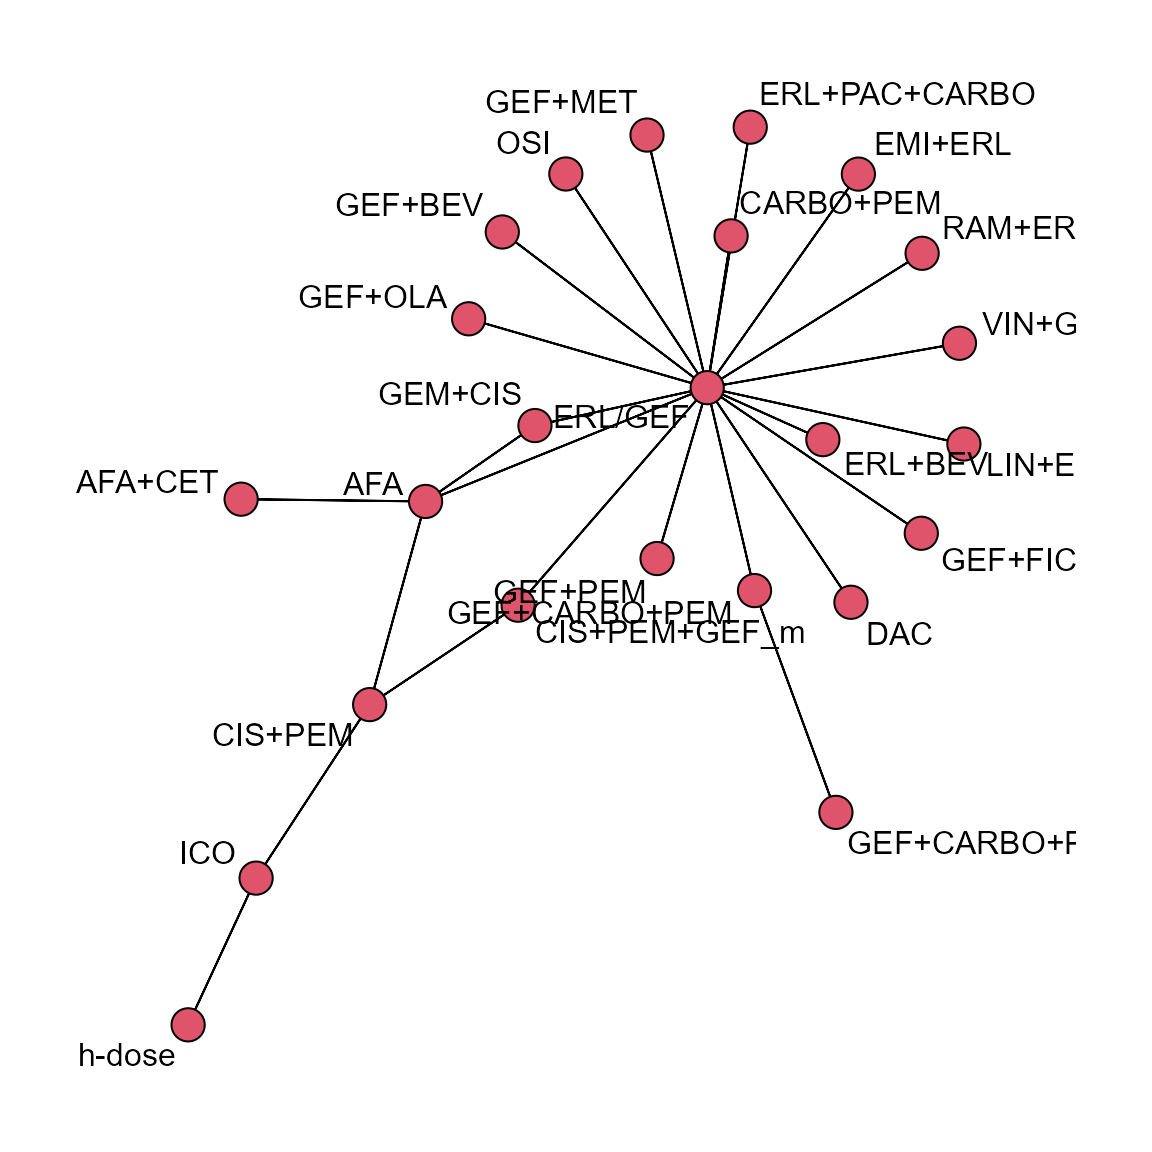
\includegraphics{how-to-use-S3_files/figure-latex/unnamed-chunk-7-1.pdf}

\hypertarget{run-mcmc}{%
\subsubsection{Run MCMC}\label{run-mcmc}}

\begin{Shaded}
\begin{Highlighting}[]
\NormalTok{nma\_res }\OtherTok{\textless{}{-}} \FunctionTok{NMA\_run}\NormalTok{(nma\_model)}
\CommentTok{\#\textgreater{} Loading required namespace: BRugs}
\CommentTok{\#\textgreater{} Welcome to BRugs connected to OpenBUGS version 3.2.3}
\CommentTok{\#\textgreater{} model is syntactically correct}
\CommentTok{\#\textgreater{} data loaded}
\CommentTok{\#\textgreater{} model compiled}
\CommentTok{\#\textgreater{} Initializing chain 1:}
\CommentTok{\#\textgreater{} initial values loaded and chain initialized but another chain contain uninitialized variables}
\CommentTok{\#\textgreater{} Initializing chain 2:}
\CommentTok{\#\textgreater{} model is initialized}
\CommentTok{\#\textgreater{} model is already initialized}
\CommentTok{\#\textgreater{} Sampling has been started ...}
\CommentTok{\#\textgreater{} 10 updates took 0 s}
\CommentTok{\#\textgreater{} deviance set}
\CommentTok{\#\textgreater{} monitor set for variable \textquotesingle{}beta\textquotesingle{}}
\CommentTok{\#\textgreater{} monitor set for variable \textquotesingle{}totresdev\textquotesingle{}}
\CommentTok{\#\textgreater{} monitor set for variable \textquotesingle{}deviance\textquotesingle{}}
\CommentTok{\#\textgreater{} 150 updates took 0 s}
\CommentTok{\#\textgreater{} Warning in dir.create(path = here(folder)): \textquotesingle{}C:\textbackslash{}Users\textbackslash{}Nathan\textbackslash{}Documents\textbackslash{}ICON\textbackslash{}NMA\textbackslash{}output\textquotesingle{} already exists}

\NormalTok{nma\_res}
\CommentTok{\#\textgreater{} Inference for Bugs model at "C:/Users/Nathan/Documents/ICON/NMA/inst/FE\_med\_bin.txt", fit using OpenBUGS,}
\CommentTok{\#\textgreater{}  2 chains, each with 160 iterations (first 10 discarded)}
\CommentTok{\#\textgreater{}  n.sims = 300 iterations saved}
\CommentTok{\#\textgreater{}            mean    sd  2.5\%   25\%   50\%   75\%  97.5\% Rhat n.eff}
\CommentTok{\#\textgreater{} beta[2]     0.2   0.7  {-}0.7  {-}0.5   0.1   0.7    1.3  2.2     4}
\CommentTok{\#\textgreater{} beta[3]    {-}0.9   0.9  {-}2.2  {-}2.0  {-}0.5  {-}0.1    0.0  7.0     2}
\CommentTok{\#\textgreater{} beta[4]     0.5   0.1   0.2   0.4   0.4   0.5    0.7  1.0   210}
\CommentTok{\#\textgreater{} beta[5]     1.4   0.6   0.1   1.2   1.4   1.8    2.3  2.0     4}
\CommentTok{\#\textgreater{} beta[6]     0.8   0.7  {-}0.2   0.4   0.9   1.1    2.8  1.5     6}
\CommentTok{\#\textgreater{} beta[7]    {-}0.5   0.1  {-}0.7  {-}0.5  {-}0.5  {-}0.4   {-}0.2  1.0   300}
\CommentTok{\#\textgreater{} beta[8]    {-}0.1   0.2  {-}0.4  {-}0.2  {-}0.1   0.0    0.2  1.0   190}
\CommentTok{\#\textgreater{} beta[9]    {-}0.5   0.1  {-}0.7  {-}0.6  {-}0.5  {-}0.4   {-}0.3  1.0   210}
\CommentTok{\#\textgreater{} beta[10]   {-}0.2   0.7  {-}1.3  {-}0.5  {-}0.2   0.1    0.7  1.2   230}
\CommentTok{\#\textgreater{} beta[11]    0.9   0.8  {-}0.6   0.4   1.0   1.4    2.2  1.1    26}
\CommentTok{\#\textgreater{} beta[12]   {-}0.7   0.1  {-}0.9  {-}0.8  {-}0.7  {-}0.6   {-}0.5  1.0   300}
\CommentTok{\#\textgreater{} beta[13]   {-}0.4   0.3  {-}0.9  {-}0.6  {-}0.4  {-}0.2    0.3  1.0   150}
\CommentTok{\#\textgreater{} beta[14]   {-}0.3   0.2  {-}0.7  {-}0.4  {-}0.3  {-}0.2    0.2  1.1    21}
\CommentTok{\#\textgreater{} beta[15]    0.0   0.2  {-}0.3  {-}0.1   0.0   0.1    0.3  1.0   110}
\CommentTok{\#\textgreater{} beta[16]   {-}0.3   0.2  {-}0.6  {-}0.4  {-}0.3  {-}0.2    0.1  1.0   300}
\CommentTok{\#\textgreater{} beta[17]   {-}0.9   0.6  {-}2.1  {-}1.5  {-}0.6  {-}0.4   {-}0.2  1.0    91}
\CommentTok{\#\textgreater{} beta[18]    1.3   0.4   0.7   0.9   1.3   1.6    1.9  2.1     4}
\CommentTok{\#\textgreater{} beta[19]    0.9   0.6  {-}0.4   0.6   0.9   1.4    1.9  2.8     3}
\CommentTok{\#\textgreater{} beta[20]    0.6   0.6  {-}0.7   0.3   0.7   1.1    1.7  2.6     3}
\CommentTok{\#\textgreater{} beta[21]    0.3   0.3  {-}0.3   0.1   0.3   0.5    0.8  1.0   300}
\CommentTok{\#\textgreater{} beta[22]   {-}0.8   0.1  {-}1.0  {-}0.8  {-}0.8  {-}0.7   {-}0.6  1.0   300}
\CommentTok{\#\textgreater{} beta[23]   {-}0.5   0.1  {-}0.8  {-}0.6  {-}0.5  {-}0.4   {-}0.3  1.0   200}
\CommentTok{\#\textgreater{} beta[24]    0.4   0.6  {-}0.7   0.0   0.3   0.8    1.4  1.2    11}
\CommentTok{\#\textgreater{} totresdev 655.5 578.3 110.6 293.6 385.8 919.6 1813.1  1.1    41}
\CommentTok{\#\textgreater{} deviance  670.8 578.7 126.9 309.2 400.9 933.8 1833.6  1.1    45}
\CommentTok{\#\textgreater{} }
\CommentTok{\#\textgreater{} For each parameter, n.eff is a crude measure of effective sample size,}
\CommentTok{\#\textgreater{} and Rhat is the potential scale reduction factor (at convergence, Rhat=1).}
\CommentTok{\#\textgreater{} }
\CommentTok{\#\textgreater{} DIC info (using the rule, pD = Dbar{-}Dhat)}
\CommentTok{\#\textgreater{} pD = 349.8 and DIC = 1021.0}
\CommentTok{\#\textgreater{} DIC is an estimate of expected predictive error (lower deviance is better).}

\CommentTok{\# diagnostics(nma\_res)}
\CommentTok{\# nma\_outputs(nma\_res)}
\end{Highlighting}
\end{Shaded}

\hypertarget{reconfigure-model}{%
\subsubsection{Reconfigure model}\label{reconfigure-model}}

It is simple to modify an existing analysis without repeating the
previous steps. For example, we can run the NMA for a random effects
model version of the same model.

\begin{Shaded}
\begin{Highlighting}[]
\NormalTok{nma\_model2 }\OtherTok{\textless{}{-}}
  \FunctionTok{NMA\_update}\NormalTok{(nma\_model,}
             \AttributeTok{is\_random =} \ConstantTok{TRUE}\NormalTok{)}

\NormalTok{nma\_res2 }\OtherTok{\textless{}{-}} \FunctionTok{NMA\_run}\NormalTok{(nma\_model2,}
                    \AttributeTok{output\_dir =} \StringTok{"RE output"}\NormalTok{)}
\CommentTok{\#\textgreater{} model is syntactically correct}
\CommentTok{\#\textgreater{} data loaded}
\CommentTok{\#\textgreater{} model compiled}
\CommentTok{\#\textgreater{} Initializing chain 1:}
\CommentTok{\#\textgreater{} initial values loaded but chain contain uninitialized variables}
\CommentTok{\#\textgreater{} Initializing chain 2:}
\CommentTok{\#\textgreater{} initial values loaded but chain contain uninitialized variables}
\CommentTok{\#\textgreater{} initial values generated, model initialized}
\CommentTok{\#\textgreater{} Sampling has been started ...}
\CommentTok{\#\textgreater{} 10 updates took 0 s}
\CommentTok{\#\textgreater{} deviance set}
\CommentTok{\#\textgreater{} monitor set for variable \textquotesingle{}beta\textquotesingle{}}
\CommentTok{\#\textgreater{} monitor set for variable \textquotesingle{}totresdev\textquotesingle{}}
\CommentTok{\#\textgreater{} monitor set for variable \textquotesingle{}deviance\textquotesingle{}}
\CommentTok{\#\textgreater{} 150 updates took 0 s}
\CommentTok{\#\textgreater{} Warning in dir.create(path = here(folder)): \textquotesingle{}C:\textbackslash{}Users\textbackslash{}Nathan\textbackslash{}Documents\textbackslash{}ICON\textbackslash{}NMA\textbackslash{}RE output\textquotesingle{} already exists}

\NormalTok{nma\_res2}
\CommentTok{\#\textgreater{} Inference for Bugs model at "C:/Users/Nathan/Documents/ICON/NMA/inst/RE\_med\_bin.txt", fit using OpenBUGS,}
\CommentTok{\#\textgreater{}  2 chains, each with 160 iterations (first 10 discarded)}
\CommentTok{\#\textgreater{}  n.sims = 300 iterations saved}
\CommentTok{\#\textgreater{}            mean    sd  2.5\%   25\%   50\%   75\%  97.5\% Rhat n.eff}
\CommentTok{\#\textgreater{} beta[2]    {-}0.6   5.4  {-}7.0  {-}6.3   0.1   4.6    5.9 12.1     2}
\CommentTok{\#\textgreater{} beta[3]    {-}5.5   3.2 {-}10.1  {-}9.2  {-}3.4  {-}2.6   {-}1.8  5.3     2}
\CommentTok{\#\textgreater{} beta[4]     0.4   1.7  {-}2.1  {-}1.5   0.9   1.9    2.8  6.3     2}
\CommentTok{\#\textgreater{} beta[5]     1.1   1.1  {-}0.9   0.4   0.7   2.3    3.1  1.7     6}
\CommentTok{\#\textgreater{} beta[6]     0.8   3.9  {-}5.4  {-}3.9   2.6   4.3    5.1  5.2     2}
\CommentTok{\#\textgreater{} beta[7]    {-}1.1   1.2  {-}3.5  {-}2.2  {-}0.9  {-}0.1    0.7  1.9     4}
\CommentTok{\#\textgreater{} beta[8]    {-}2.2   0.9  {-}3.7  {-}2.9  {-}2.3  {-}1.7   {-}0.1  1.0   300}
\CommentTok{\#\textgreater{} beta[9]    {-}0.9   1.0  {-}2.8  {-}1.3  {-}0.7  {-}0.2    0.7  1.2    26}
\CommentTok{\#\textgreater{} beta[10]   {-}1.8   1.3  {-}3.6  {-}2.6  {-}2.2  {-}0.9    0.9  3.5     3}
\CommentTok{\#\textgreater{} beta[11]    2.0   1.3  {-}1.0   1.3   2.2   2.9    4.3  1.1    15}
\CommentTok{\#\textgreater{} beta[12]   {-}1.2   0.5  {-}2.0  {-}1.5  {-}1.3  {-}1.0   {-}0.3  2.0     4}
\CommentTok{\#\textgreater{} beta[13]   {-}2.6   2.2  {-}6.5  {-}3.8  {-}2.5  {-}0.8    0.8  3.6     3}
\CommentTok{\#\textgreater{} beta[14]   {-}0.7   1.1  {-}2.1  {-}1.5  {-}1.0   0.2    1.6  1.9     4}
\CommentTok{\#\textgreater{} beta[15]    0.1   1.2  {-}2.0  {-}0.8  {-}0.1   1.1    2.2  3.4     3}
\CommentTok{\#\textgreater{} beta[16]    1.7   0.8   0.0   1.1   1.8   2.4    2.9  1.0   260}
\CommentTok{\#\textgreater{} beta[17]    3.2   3.0  {-}0.3   0.6   0.8   6.2    7.8  4.0     2}
\CommentTok{\#\textgreater{} beta[18]    0.8   2.1  {-}2.4  {-}1.1   0.7   2.6    4.4  6.2     2}
\CommentTok{\#\textgreater{} beta[19]    1.7   2.4  {-}1.2  {-}0.5   0.8   4.4    5.3  6.0     2}
\CommentTok{\#\textgreater{} beta[20]    1.4   1.3  {-}0.7   0.3   1.5   2.6    3.7  4.3     2}
\CommentTok{\#\textgreater{} beta[21]    2.0   1.5  {-}1.7   1.2   2.2   3.2    4.3  1.2    24}
\CommentTok{\#\textgreater{} beta[22]    1.3   1.5  {-}0.5   0.2   0.7   2.8    4.3  2.7     3}
\CommentTok{\#\textgreater{} beta[23]   {-}2.3   1.0  {-}3.8  {-}2.9  {-}2.5  {-}1.9    0.0  1.7     5}
\CommentTok{\#\textgreater{} beta[24]    0.5   1.2  {-}1.7  {-}0.5   0.7   1.7    2.3  3.8     2}
\CommentTok{\#\textgreater{} totresdev 423.5 398.4  69.8 104.6 394.6 580.1 1670.6  5.3     2}
\CommentTok{\#\textgreater{} deviance  440.8 401.0  84.7 121.1 412.8 594.5 1699.7  5.3     2}
\CommentTok{\#\textgreater{} }
\CommentTok{\#\textgreater{} For each parameter, n.eff is a crude measure of effective sample size,}
\CommentTok{\#\textgreater{} and Rhat is the potential scale reduction factor (at convergence, Rhat=1).}
\CommentTok{\#\textgreater{} }
\CommentTok{\#\textgreater{} DIC info (using the rule, pD = Dbar{-}Dhat)}
\CommentTok{\#\textgreater{} pD = 216.0 and DIC = 656.8}
\CommentTok{\#\textgreater{} DIC is an estimate of expected predictive error (lower deviance is better).}

\CommentTok{\# diagnostics(nma\_res2, save = TRUE)}
\CommentTok{\# nma\_outputs(nma\_res2, save = TRUE)}
\end{Highlighting}
\end{Shaded}


\end{document}
